% Adjust these for the path of the theme and its graphics, relative to this file
\usepackage{../../beamerthemeFalmouthGamesAcademy}
\usepackage{multimedia}
\usepackage{soul}
\graphicspath{ {../../} }

% Default language for code listings
\lstset{language=C++,
        morekeywords={each,in,nullptr}
}

% For strikethrough effect
\usepackage[normalem]{ulem}
\usepackage{wasysym}

\usepackage{pdfpages}

% http://www.texample.net/tikz/examples/state-machine/
\usetikzlibrary{arrows,automata}

\newcommand{\modulecode}{COMP260}\newcommand{\moduletitle}{Distributed Systems}\newcommand{\sessionnumber}{5}

\begin{document}
\title{\sessionnumber: Human-Centred Design}
\subtitle{\modulecode: \moduletitle}

\frame{\titlepage} 

% LEARNING OUTCOMES
\begin{frame}
	\frametitle{Learning outcomes:}
	\begin{itemize}
		\item \textbf{explain} the importance of placing the user at the centre of the design process
		\item \textbf{briefly} describe and compare different user-centred design techniques
		\item \textbf{demonstrate} a knowledge o the principles of user-centred design.	
	\end{itemize}
\end{frame}

\begin{frame}
	\frametitle{A Word of Warning}
	AR/VR are both emerging technologies and thus they borrow language from other similar disciplines such as game development, film studies and 3D design. This appropriation of lexicons can be confusing and there will be some overlap in relation to key terms and definitions.
\end{frame}

% HUMAN CENTRED DESIGN
\begin{frame}
	\frametitle{Human-Centred Design (HCD)}
	
	Sophisticated / eloquent technical solutions are less important than great user experiences.
\end{frame}

% CONTINUOUS DISCOVERY 
\begin{frame}
	\frametitle{Continuous Discovery}
	Continuous discovery is the on-going process of engaging users during the design and development process. 
	\begin{itemize}
		\item \pause You can never know everything in advance of a project.
		\item \pause Waiting until the end of a build to find out that something doesn't work is unsustainable. 
		\item \pause Change is inevitable.
		\item \pause Failures are an inevitable outcome of creativity and innovation. 
	\end{itemize}
\end{frame}	

% ITERATION CYCLE
\begin{frame}
	\frametitle{Iteration}
	\begin{figure}
		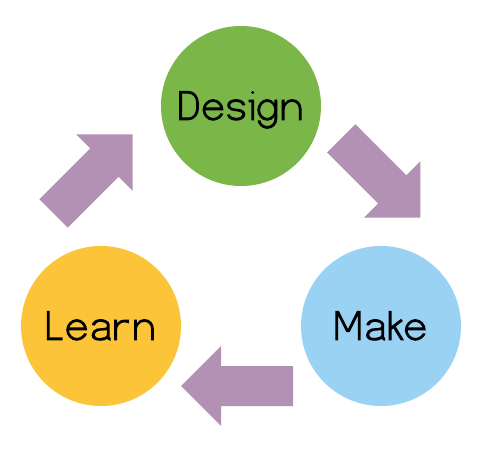
\includegraphics[scale=0.4]{assets/iteration.png}
		\caption{The Iteration Cycle}
	\end{figure}
\end{frame}


% DEFINE STAGE
\begin{frame}
	\frametitle{ \st{Design} Define Stage}
	This stage attempts to answer the question, `what do we want to make?' and includes everything from the high-level vision to listing requirements.
	\pause
	\begin{columns}
		\begin{column}{0.5\textwidth}
			\begin{itemize}
				\item Vision
				\item Objectives 
				\item Key Players				
				\item Time \& Costs
				\item Risks
			\end{itemize}
   		\end{column}
		
		\begin{column}{0.5\textwidth}  
			\begin{itemize}
				\item Assumptions
				\item Constraints
				\item Personas		
				\item User Stories
				\item Story Boards
			\end{itemize}
		\end{column}
	\end{columns}
\end{frame}

\begin{frame}
	\frametitle{\textbf{ASK QUESTIONS}}
	\begin{itemize}
		\item Feedback is crucial at the define stage. 
		\item Ask lots of questions.
		\item Do not trust assumptions. 
		\item Common misconception.
	\end{itemize}
\end{frame}

\begin{frame}
	\begin{center}
		\Huge{Analysis Paralysis }
	\end{center}
\end{frame}


% MAKE STAGE
\begin{frame}
	\frametitle{Make Stage}
	This stage answers the question, `how do we make it?' and then proceeds to make it 
\end{frame}



\begin{frame}
	\begin{itemize}
		\item \textbf{Design Stage} - this stage attempts to answer the question, ?what do we make?? and includes everything from the high-level vision to listing requirements. 
		\item \textbf{Make Stage} - This stage answers the question, ?how do we make it?? and then proceeds to make it. 
		\item \textbf{Learn Stage} - This stage answers the question, ?what works and what does not work?? the answers are fed back into the define stage to refine what is to be made. 
	\end{itemize}
\end{frame}



	
\end{document}
